
\documentclass[10pt]{IEEEtran}
\pdfoutput=1

\usepackage{graphicx}
\usepackage{hyperref}
\usepackage[utf8]{inputenc}
\usepackage{listings}
\usepackage[table]{xcolor}
\usepackage{pdfpages}

\hypersetup{colorlinks=true,citecolor=[rgb]{0,0.4,0}}


\title{Predictive Beer Analytics}
\author{Joshua Weinstein, Jim Sundkvist, Marek Kühn}

\begin{document}
\maketitle

\begin{abstract}
This project aims to apply various concepts of Python programming as well as data mining and processing.
Based on a large amount of user and beer data, the application uses varying techniques including data mining, natural language processing, and color analysis to predict user-defined beers' desirability in the world through a web application. 
\end{abstract}

\section{Introduction}

The Predictive Beer Analytics project has been initiated in the Fall of 2014 as a part of "\textit{Data Mining Using Python}" course at Denmark Technical University. Its purpose is not only exercise the study material, but also to give users some useful, informative results. To satisfy this, we used our previous experience with web development and created a lightweight web-service with visual representations of the results. The users can design their own beer by defining its style, alcohol by volume, keywords and dominant label color. This information is then used to generate a desirability map (ref).

The application to retrieve and analyse data along with our web application (without the database) can be found on our GitHub account. The web-service can be run locally with an installation of Django, MySQL, and a copy of the database.

\section{Data mining}
Being the main aspect of any data mining project, retrieving the data, and a lot of it, is the first course of action. All data used by Predictive Beer Analytics was gathered through the \textit{Untappd API}, a beer review website which provides access to the data it collects. Unfortunately, the service limited our access to their data to 100 calls an hour. This significantly increased the amount of time required to gather data. The script, \texttt{untappd.py} provides data structures to store Untappd data as well as uses the \textit{Requests} module to make calls to Untappd's servers. Due to the available requests through the API service, it was necessary to first retrieve a list of active users and then later use their username to gather information about beer they have reviewed in the past. Over the course of roughly two weeks of mining, a reasonable amount of information was stored. Seen in figure \ref{fig:dataQuantity}, over 200.000 user reviews are used to predict the desirability of a beer based on location. To keep this information up-to-date, \texttt{dataQuantity.py} script has been included in the library. 

\begin{figure}[h]
  \centering
  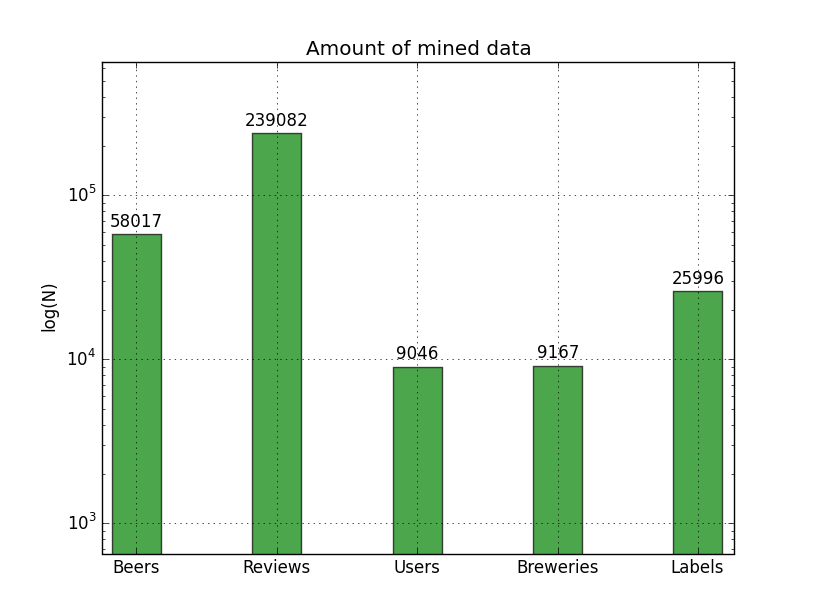
\includegraphics[width=\columnwidth]{./graphics/quantity.png}
  \caption{Amount of used data (by the time of presentation)}
  \label{fig:dataQuantity}
\end{figure}

After data has been gathered, updated, and normalized with methods in the main script \texttt{predictiveBeerAnalytics.py}, it is split up into users and beers where users contain a location and their ratings and beers are composed of descriptive keywords, alcohol content, label's location, style, and other unused information. These are then used in conjunction with other scripts we have written to analyse label colors, determine keywords from descriptions, find relationships between alcohol content and location, and  determining relationships between a user's location and the style of beer they enjoy.

\section{Machine learning}
There are two applications of machine learning: 

\begin{itemize}
  \item \textbf{Natural language processing}
  \item \textbf{Image color analysis}
\end{itemize}

With its extraordinary lexical resources and easy-to-use interface, \textbf{Natural Language Toolkit (NLTK)} was an easy choice. It is used to tokenize the sentence in order to classify the words according to its type. After various filtering, we calculate the average rating of each keyword. The best, worst and the most used keywords are presented on the website. The relevance of the results is to be discussed later.

While thinking about all aspects that can possibly affect the beer desirability, we introduced also the visual point of view. We have no information about the color of the bottle. Nevertheless, more than half of the beers from untappd have a link to the beer label picture attached. All we had to do is determine how the beers are rated in relation to the label color. The extraction of the dominant colors is done with \textbf{sklearn.cluster} module, built on \textbf{NumPy}, \textbf{SciPy}, and \textbf{matplotlib} open-source libraries. All of which are also used regularly in other context in this project. Currently, we use K-means clustering algorithm to determine five of the most used colors in each label. The class responsible for the calculations is designed such as the parameters like number of clustered colors are easy to change in the future.

To check if the result is correct, we use the clustered colors to rebuild the picture as in the figure \ref{fig:colorClustering}. Since we observed a lot of labels not having rectangular shape, we made a custom masking algorithm based on the color differences. 

\begin{figure}[b]
  \centering
  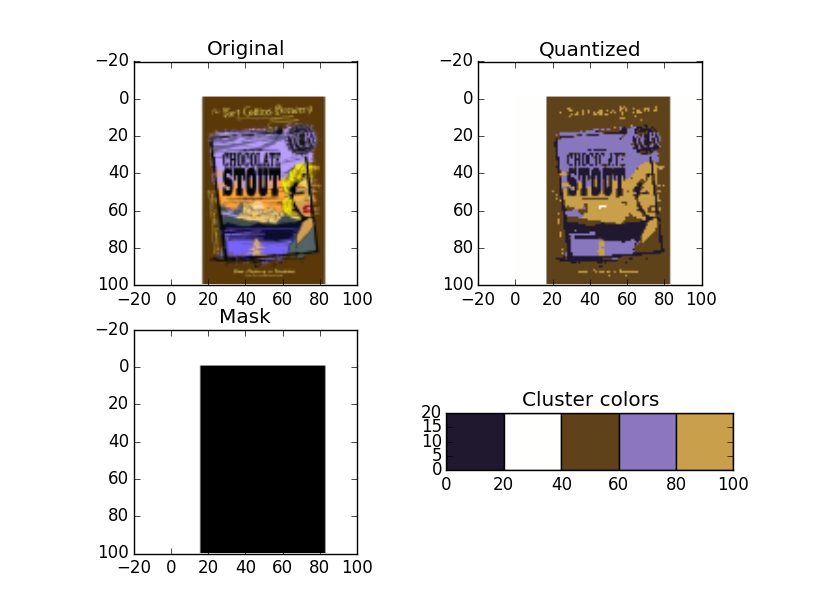
\includegraphics[width=\columnwidth]{./graphics/1.png}
  \caption{Image color clustering}
  \label{fig:colorClustering}
\end{figure}

Having these colors extracted, they need to be associated with ratings. Otherwise there would be no measurable impact on the total beer desirability. We couldn't match those color directly to the user input, because that way its rating would have to be calculated  every time the request is made, which is not acceptable given the amount of data. So we come up with a solution by using template color palette. It serves as a fixed categorizing root. None of the available functions were suitable for comparing the RGB values of the colors, so we designed our own classification algorithm. It uses the well-known euclidean distance formula to determine which color from the template color palette is the closest. However, simple distance in RGB colorspace doesn't correspond to human perception. A change of one parameter results in much more different color than the same change distributed between multiple parameters. It was possible to overcome this by converting the colors to YUV colorspace (Fig. \ref{fig:colorspace}), which takes human perception into account, making the response more or less linear. 


\begin{figure}[t]
  \centering
  
\includegraphics[width=6cm]{./graphics/YUV.png}
  \caption{YUV linear colorspace sample for Y = 0}
  \label{fig:colorspace}
\end{figure}

\section{Web service}

The web-service uses one of the most popular Python frameworks - Django. This allowed us to create elegant web application while still being able to focus on the server-side python scripts rather than web-design. 

HACKPROOF no cross-site-scripting HAHA

\section{Discussion}

Keywords - Regular expression.

Hardcoded web color palette

\section{Further development}
Collecting data

Machine learning

Website

Including brewery information








Lorem ipsum dolor sit amet, consectetur adipisicing elit, sed do
eiusmod tempor incididunt ut labore et dolore magna aliqua. Ut enim ad
minim veniam, quis nostrud exercitation ullamco laboris nisi ut
aliquip ex ea commodo consequat. Duis aute irure dolor in
reprehenderit in voluptate velit esse cillum dolore eu fugiat nulla
pariatur. Excepteur sint occaecat cupidatat non proident, sunt in
culpa qui officia deserunt mollit anim id est laborum.

Lorem ipsum dolor sit amet, consectetur adipisicing elit, sed do
eiusmod tempor incididunt ut labore et dolore magna aliqua. Ut enim ad
minim veniam, quis nostrud exercitation ullamco laboris nisi ut
aliquip ex ea commodo consequat. Duis aute irure dolor in
reprehenderit in voluptate velit esse cillum dolore eu fugiat nulla
pariatur. Excepteur sint occaecat cupidatat non proident, sunt in
culpa qui officia deserunt mollit anim id est laborum.

Lorem ipsum dolor sit amet, consectetur adipisicing elit, sed do
eiusmod tempor incididunt ut labore et dolore magna aliqua. Ut enim ad
minim veniam, quis nostrud exercitation ullamco laboris nisi ut
aliquip ex ea commodo consequat. Duis aute irure dolor in
reprehenderit in voluptate velit esse cillum dolore eu fugiat nulla
pariatur. Excepteur sint occaecat cupidatat non proident, sunt in
culpa qui officia deserunt mollit anim id est laborum.

Lorem ipsum dolor sit amet, consectetur adipisicing elit, sed do
eiusmod tempor incididunt ut labore et dolore magna aliqua. Ut enim ad
minim veniam, quis nostrud exercitation ullamco laboris nisi ut
aliquip ex ea commodo consequat. Duis aute irure dolor in
reprehenderit in voluptate velit esse cillum dolore eu fugiat nulla
pariatur. Excepteur sint occaecat cupidatat non proident, sunt in
culpa qui officia deserunt mollit anim id est laborum.

The web service is a single CGI script and the listing begins at page
\pageref{listing:brede_str_nmf}. 

\section{Results}


Figure~\ref{fig:topicsentiment} shows a screenshot of the webservice
with data copy-and-pasted from the
\href{http://en.wikipedia.org/wiki/Lundbeck}{Wikipedia article on
  Lundbeck}. 

Lorem ipsum dolor sit amet, consectetur adipisicing elit, sed do
eiusmod tempor incididunt ut labore et dolore magna aliqua. Ut enim ad
minim veniam, quis nostrud exercitation ullamco laboris nisi ut
aliquip ex ea commodo consequat. Duis aute irure dolor in
reprehenderit in voluptate velit esse cillum dolore eu fugiat nulla
pariatur. Excepteur sint occaecat cupidatat non proident, sunt in
culpa qui officia deserunt mollit anim id est laborum.

Lorem ipsum dolor sit amet, consectetur adipisicing elit, sed do
eiusmod tempor incididunt ut labore et dolore magna aliqua. Ut enim ad
minim veniam, quis nostrud exercitation ullamco laboris nisi ut
aliquip ex ea commodo consequat. Duis aute irure dolor in
reprehenderit in voluptate velit esse cillum dolore eu fugiat nulla
pariatur. Excepteur sint occaecat cupidatat non proident, sunt in
culpa qui officia deserunt mollit anim id est laborum.

\subsection{Code checking}

We used \href{http://www.logilab.org/857}{pylint} to check our coding
quality. 

Lorem ipsum dolor sit amet, consectetur adipisicing elit, sed do
eiusmod tempor incididunt ut labore et dolore magna aliqua. Ut enim ad
minim veniam, quis nostrud exercitation ullamco laboris nisi ut
aliquip ex ea commodo consequat. Duis aute irure dolor in
reprehenderit in voluptate velit esse cillum dolore eu fugiat nulla
pariatur. Excepteur sint occaecat cupidatat non proident, sunt in
culpa qui officia deserunt mollit anim id est laborum.


\subsection{Testing}

We wrote a script that called the webscript and checked the returned
result. 

Lorem ipsum dolor sit amet, consectetur adipisicing elit, sed do
eiusmod tempor incididunt ut labore et dolore magna aliqua. Ut enim ad
minim veniam, quis nostrud exercitation ullamco laboris nisi ut
aliquip ex ea commodo consequat. Duis aute irure dolor in
reprehenderit in voluptate velit esse cillum dolore eu fugiat nulla
pariatur. Excepteur sint occaecat cupidatat non proident, sunt in
culpa qui officia deserunt mollit anim id est laborum. 


\subsection{Profiling}


Lorem ipsum dolor sit amet, consectetur adipisicing elit, sed do
eiusmod tempor incididunt ut labore et dolore magna aliqua. Ut enim ad
minim veniam, quis nostrud exercitation ullamco laboris nisi ut
aliquip ex ea commodo consequat. Duis aute irure dolor in
reprehenderit in voluptate velit esse cillum dolore eu fugiat nulla
pariatur. Excepteur sint occaecat cupidatat non proident, sunt in
culpa qui officia deserunt mollit anim id est laborum.


\section{Discussion}

With the sentiment wordlist the sentiment analysis will only work for
English texts.

There are numerous issue with the implementation: The HTML templates
are not appropriately separated from the code, the functions {\tt
  components2html\_*} have redundant code, a variable called {\tt
  wordsfreq} could be implemented as a
\href{http://docs.python.org/dev/library/collections#collections.Counter}{\tt
  collections.Counter}, etc. 
Obviously unit testing could have be done if the code was well
structured into modules, e.g., with the
\href{https://nose.readthedocs.org/en/latest/}{\tt nose} module. 
The simple word tokenization with the regular expression ``\verb!\w+!''
faults for some words, e.g., ``won't'' is tokenized to the two tokens ``won'' and
``t'' and as ``won'' is positive in the AFINN word list a positive
bias is introduced. 

There are different sparse matrix representations in scipy.sparse
(\href{http://docs.scipy.org/doc/scipy/reference/generated/scipy.sparse.csr_matrix.html}{csr}, 
\href{http://docs.scipy.org/doc/scipy/reference/generated/scipy.sparse.csc_matrix.html}{csc}
and 
\href{http://docs.scipy.org/doc/scipy/reference/generated/scipy.sparse.lil_matrix.html}{lil}). 
A proper profiling may have shown that the ``lil'' format used to set up
the matrix is not the most efficient in the iterative algorithm and
the
\href{http://docs.scipy.org/doc/scipy/reference/generated/scipy.sparse.lil_matrix.html}{documentation
  suggests} ``once a matrix has been constructed, convert to CSR or
CSC format for fast arithmetic and matrix vector operations''.
Furthermore, it is not clear how well sparse matrices works in
conjunction with dense matrices: Should {\tt W} and {\tt H} in the
{\tt nmf} function have been made sparse too?

Lorem ipsum dolor sit amet, consectetur adipisicing elit, sed do
eiusmod tempor incididunt ut labore et dolore magna aliqua. Ut enim ad
minim veniam, quis nostrud exercitation ullamco laboris nisi ut
aliquip ex ea commodo consequat. Duis aute irure dolor in
reprehenderit in voluptate velit esse cillum dolore eu fugiat nulla
pariatur. Excepteur sint occaecat cupidatat non proident, sunt in
culpa qui officia deserunt mollit anim id est laborum.


\section{Conclusion}

We implemented a fast on-the-fly topic-sentiment mining web service suitable
for small corpora.


\bibliographystyle{IEEEtran}
\bibliography{lyngby}


\clearpage
\onecolumn
\appendices
\section{Code listings}

\definecolor{darkgreen}{rgb}{0, 0.4, 0}
\lstset{language=Python,
  numbers=left,
  frame=bottomline,
  basicstyle=\scriptsize,
  identifierstyle=\color{blue},
  keywordstyle=\bfseries,
  commentstyle=\color{darkgreen},
  stringstyle=\color{red},
  literate={Ö}{{\"O}}1 {é}{{\'e}}1 {Å}{{\AA}}1,
}
\lstlistoflistings

\label{listing:PBA}\lstinputlisting{../machine_learning/lib/predictiveBeerAnalytics.py}

\label{listing:Untappd}\lstinputlisting{../machine_learning/lib/untappd.py}

\label{listing:keywordExtractor}\lstinputlisting{../machine_learning/lib/keywordExtractor.py}

\label{listing:keywordClassifier}\lstinputlisting{../machine_learning/lib/keywordClassifier.py}

\label{listing:dataPoints}\lstinputlisting{../machine_learning/lib/dataPoints.py}

\label{listing:PBAMap}\lstinputlisting{../machine_learning/lib/PBAMap.py}

\label{listing:labels}\lstinputlisting{../machine_learning/lib/labels.py}

\label{listing:fileReader}\lstinputlisting{../machine_learning/lib/fileReader.py}

\label{listing:dataQuantity}\lstinputlisting{../machine_learning/lib/dataQuantity.py}


\newpage
\section{Automatic generation of documentation}

Demontration using epydoc:
\begin{verbatim}
epydoc --pdf -o /home/fnielsen/tmp/epydoc/ --name RBBase wikipedia/api.py
\end{verbatim}
This example does not use \verb!brede_str_nmf! but another more
well-documented module called {\tt api.py} that are used to download
material from Wikipedia. 

%\includepdf[pages={-}]{/home/fnielsen/tmp/epydoc/api.pdf}

\end{document}
